\documentclass[a4paper]{article}
\usepackage[pdftex]{hyperref}
\usepackage[latin1]{inputenc}
\usepackage[english]{babel}
\usepackage{a4wide}
\usepackage{amsmath}
\usepackage{amssymb}
\usepackage{algorithmic}
\usepackage{algorithm}
\usepackage{ifthen}
\usepackage{listings}
% move the asterisk at the right position
\lstset{basicstyle=\ttfamily,tabsize=4,literate={*}{${}^*{}$}1}
%\lstset{language=C,basicstyle=\ttfamily}
\usepackage{moreverb}
\usepackage{palatino}
\usepackage{multicol}
\usepackage{tabularx}
\usepackage{comment}
\usepackage{verbatim}
\usepackage{color}

%% pdflatex?
\newif\ifpdf
\ifx\pdfoutput\undefined
\pdffalse % we are not running PDFLaTeX
\else
\pdfoutput=1 % we are running PDFLaTeX
\pdftrue
\fi
\ifpdf
\usepackage[pdftex]{graphicx}
\else
\usepackage{graphicx}
\fi
\ifpdf
\DeclareGraphicsExtensions{.pdf, .jpg}
\else
\DeclareGraphicsExtensions{.eps, .jpg}
\fi

\parindent=0cm
\parskip=0cm

\setlength{\columnseprule}{0.4pt}
\addtolength{\columnsep}{2pt}

\addtolength{\textheight}{5.5cm}
\addtolength{\topmargin}{-26mm}
\pagestyle{empty}

%%
%% Sheet setup
%% 
\newcommand{\coursename}{Machine Learning}
 
\newcommand{\sheettitle}{Homework}
\newcommand{\mytitle}{}
\newcommand{\mytoday}{\textcolor{blue} May 26, 2018}

% Current Assignment number
\newcounter{assignmentno}
\setcounter{assignmentno}{11}

% Current Problem number, should always start at 1
\newcounter{problemno}
\setcounter{problemno}{1}

%%
%% problem and bonus environment
%%
\newcounter{probcalc}
\newcommand{\problem}[2]{
  \pagebreak[2]
  \setcounter{probcalc}{#2}
  ~\\
  {\large \textbf{Problem \textcolor{blue}{\arabic{assignmentno}}.\textcolor{blue}{\arabic{problemno}}} \hspace{0.2cm}\textit{#1}} \refstepcounter{problemno}\vspace{2pt}\\}

\newcommand{\bonus}[2]{
  \pagebreak[2]
  \setcounter{probcalc}{#2}
  ~\\
  {\large \textbf{Bonus Problem \textcolor{blue}{\arabic{assignmentno}}.\textcolor{blue}{\arabic{problemno}}} \hspace{0.2cm}\textit{#1}} \refstepcounter{problemno}\vspace{2pt}\\}

%% some counters  
\newcommand{\assignment}{\arabic{assignmentno}}

%% solution  
\newcommand{\solution}{\pagebreak[2]{\bf Solution:}\\}

%% Hyperref Setup
\hypersetup{pdftitle={Homework \assignment},
  pdfsubject={\coursename},
  pdfauthor={},
  pdfcreator={},
  pdfkeywords={Machine Learning},
  %  pdfpagemode={FullScreen},
  %colorlinks=true,
  %bookmarks=true,
  %hyperindex=true,
  bookmarksopen=false,
  bookmarksnumbered=true,
  breaklinks=true,
  %urlcolor=darkblue
  urlbordercolor={0 0 0.7}
}

\begin{document}
\coursename \\
Jacobs University Bremen \hfill \mytoday\\
Mohit Shrestha\\
Seongjin Bien\hfill
\vspace*{0.3cm}\\
\begin{center}
{\Large \sheettitle{} \textcolor{blue}{\assignment}\\}
\end{center}
The multi-layer perceptron structure for the XOR classifier model was chosen according to the suggestion given in the homework file (one hidden layer with 2 neurons, bias unit in input and hidden layer, and logistic sigmoid for activation function). The input data set was simply the standard XOR input, that is, [0,0], [0,1], [1,0], and [1,1]. The validation dataset was same as the training dataset listed above.\\

We created a loop for running the training algorithm with varying step size, decreasing the size every loop from a range of 0.2 to 0.001. As we had only 4 input data to deal with, the maximum number of epochs was set at 5000 in order to compensate for that lack of data. We stopped the function once the unprocessed quadratic error $\sqrt{(training result - real result)^2})$ went below 5\% and noted down the epoch at which the rate was reached in order to find the step size that converges most quickly. An example of the result is shown in the table below:\\
\begin{center}
\begin{tabular}{| c | c |} \hline
	Step Rate & Epoch No. \\\hline
	0.2 & 1480 \\
	0.19 & 2290 \\
	0.17 & 1890 \\
	0.13 & 2520 \\
	0.12 & 3090 \\
	0.11 & 2650 \\
	0.1 & 3350 \\
	0.09 & 4170 \\
	0.07 & 4230 \\ \hline
\end{tabular}
\end{center}

Trainings that could not reach the target error rate of 5\% within 10000 epochs were not stored. This algorithm was repeated 5 times in order to verify that the result was consistent, and we found that the step size of 0.2 was the quickest, although the result was not consistent. We believe that this is due to the luck involved in setting the connection weights to a small random value: if the random value is located at a good spot, the error rate will quickly converge to below 5\%, but if it is at a bad spot, the error rate will never converge and remain stuck at around 50\%. The relatively large optimum step size can also be attributed to the simple structure of our MLP. With relatively few dimensions, there is less chance that the large step towards negative gradient will skip over a good trough. Supporting this argument is the optimum step size we found for the MLP used in the extra task $f:[-1,1]^2 \rightarrow \{0,1\}$, with much bigger structure. \\
Throughout the process, we tracked the error rate after every 5 epochs against the validation dataset (remember, same as the training dataset) for both unprocessed and processed output. For processing the output, we simply used this function:
\begin{lstlisting}
	def output_process(x):
		if(x <= 0.5):
			return 0
		else:
			return 1
\end{lstlisting}
A graph of the error convergence rate for the best-performing model at step size = 0.2 is shown below, with results truncated at 5000 epochs for brevity: 
\begin{center}
	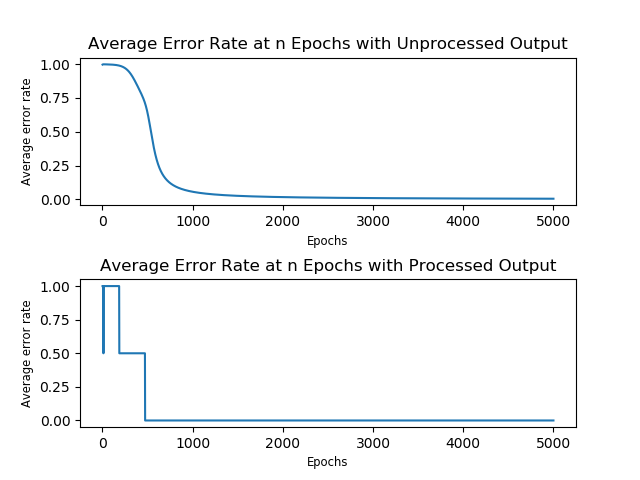
\includegraphics[scale=0.4]{res.png}\\
	Figure 1. Average Error Rate of XOR MLP Classifier at n Epochs with Two Types of Output \\
\end{center}
It can be easily seen that both the raw and processed output of the model quickly converges to 0\% error rate. \\
We decided to design a MLP for the continuous version of the same problem, $f:[-1,1]^2 \rightarrow \{0,1\}$ with $f(x,y) = sign(x,y)$. Once again, we created a nested loop for testing different number of neurons in the hidden layer (from 2 to 20) and the step sizes used to train the model. During the training, however, we discovered that the logistic sigmoid we used for the activation function suffered from precision overflow error. Both tasks were coded in Python with Numpy, so we do not know whether this problem is also present in Matlab. To deal with the issue, we decided to use the hyperbolic tangent instead, as it does not suffer from the same problem. \\
Both the training and validation dataset was generated using the following loop:
\begin{lstlisting}
	X = []
	Y = []
	for i in range(0, 1000):
		x1 = random.uniform(-1,1)
		x2 = random.uniform(-1,1)
		X.append(x1, x2)
		Y.append(np.sign(x1*x2))
\end{lstlisting}
Since there were 1000 data points to train the model from, much richer than the XOR dataset we used in the previous assignment, we set the maximum epoch limit to 200. Again, throughout the training, we tracked the processed quadratic error (it allowed the calculation to be terminated a little more quickly than the unprocessed quadratic error) of the algorithm and stopped the iteration once the error rate fell below the error threshold of 10\%. For processing the data, we used the following function: \\
\begin{lstlisting}
def output_process(x):
   if(x < 0):
       return -1
   elif(x == 0):
       return 0
   else:
       return 1
\end{lstlisting}
After repeating the whole process 5 times, each time with a newly generated training and validation dataset, we determined that the step size of 0.005 with 10 hidden layer neurons yielded a good convergence rate. An example of one such loop can be seen in the table below:\\
\begin{center}
	\begin{tabular}{| c | c |}\hline
		Step Rate & Epoch \\\hline
		0.015 & 35\\
		0.014 & 15\\
		0.013 & 30\\
		0.012 & 55\\
		0.011 & 30\\
		0.01 & 20\\
		0.009 & 30\\
		0.008 & 40\\
		0.007 & 20\\
		0.006 & 50\\
		0.005 & 20\\
		0.004 & 25\\
		0.003 & 40\\
		0.002 & 20\\\hline
	\end{tabular}
\end{center}
We also plotted the average error rate against epochs for the best model (step size = 0.005, hidden layer neuron \# = 10) The result of the training is shown below:
\begin{center}
	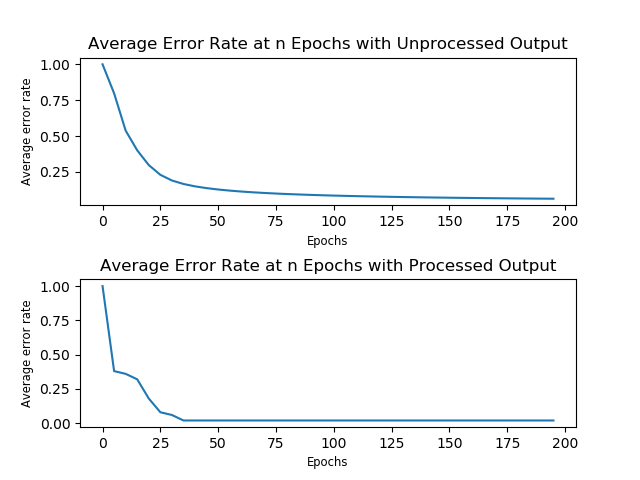
\includegraphics[scale=0.5]{resextra.png}\\
	Figure 2. Average Error Rate of sign(xy) MLP Classifier at n Epochs with Two Types of Output
\end{center}
We then another set of 100 validation data points with the model, and plotted the processed output against the input in Matlab. While the sign function returns -1, 0, or 1 depending on the input, since the task demanded the output to be Boolean, we first processed the output using the following function:
\begin{lstlisting}
def process_result(x):
   if(x <= 0):
       return 0
   else:
       return x
\end{lstlisting}
The 3D scatter plot can be seen in the image below.\\
\begin{center}
	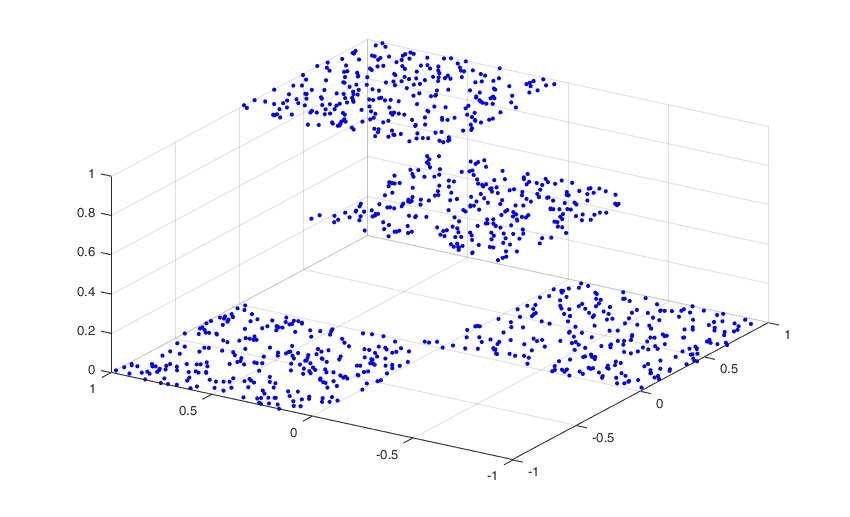
\includegraphics[scale=0.4]{index.jpg}\\
	Figure 3: 3D Scatter Plot of the sign(xy) Function with MLP
\end{center}
It can be easily seen that the output is almost perfect, save for a few edge cases very close to the boundaries (the points near the [0, 0, 1]).

\end{document}
